%!xelatex = 'xelatex --halt-on-error %O %S'

\documentclass{thuemp}
\begin{document}

% 标题,作者
\emptitle{Homework 6}
\empauthor{江灿}{2019011325}

% 奇数页页眉 % 请在这里写出第一作者以及论文题目
\fancyhead[CO]{{\footnotesize 江灿: 清华大学算法分析与设计基础}}

\maketitle

\noindent\rule[0.25\baselineskip]{\textwidth}{1pt}
%%%%%%%%%%%%%%%%%%%%%%%%%%%%%%%%%%%%%%%%%%%%%%%%%%%%%%%%%%%%%%%%
%  正文由此开始
%%%%%%%%%%%%%%%%%%%%%%%%%%%%%%%%%%%%%%%%%%%%%%%%%%%%%%%%%%%%%%%%
\wuhao 

\section*{15.1-3 Consider a modification of the rod-cutting problem in which, in addition to a price pifor each rod, each cut incurs a fixed cost of c. The revenue associated with a solution is now the sum of the prices of the pieces minus the costs of making the cuts. Give a dynamic-programming algorithm to solve this modified problem.}

${MODIF-ROD-CUTTING(p,n,c) }$
\begin{lstlisting}
if n==0
	return 0
q = -∞
for i = i to n
	q = max(q,p[i] + MODIF-ROD-CUTTING(p,n - i,c) - c)
return q
\end{lstlisting}
增添一个c在进行比较的时候即可
\section*{15.3-4 As stated, in dynamic programming we first solve the subproblems and then choose which of them to use in an optimal solution to the problem. Professor Capulet claims that we do not always need to solve all the subproblems in order to find an optimal solution. She suggests that we can find an optimal solution to the matrixchain multiplication problem by always choosing the matrix ··· suboptimal solution.}
找一个使用该算法,但是不是最优解的即可。
该算法与动态规划的差别在与
\[ q =\min\{ q,m[i,k] + m[k + 1, j] + p_{i-1}p_kp_j\}\]
比较的时候,没有对于考虑到m[i,k] + m[k + 1, j]而是直接选取最小的p\\
显然,会存在$ p_{i-1}p_kp_j$最小,但是$m[i,k] + m[k + 1, j] + p_{i-1}p_kp_j$不是最小的情况,如:
\begin{equation*}
	\begin{split}
	Maxtrix \ size : 1\times 8,8\times 21,21\times 7, 7\times 20, 20\times 18, 18\times 1,1\times 8,8 \times 1\\
	while\ the\ greedy:(((((((A_0A_1)A_2)A_3)A_4)A_5)A_6)A_7)\ which \ cost =849\\
	but\ the \ optimal \ is: ((((A_0A_1)A_2)(A_3(A_4A_5)))(A_6A_7))\ which \ cost =831
\end{split}
\end{equation*}
% \begin{figure}[H]
% 	\centering
% 	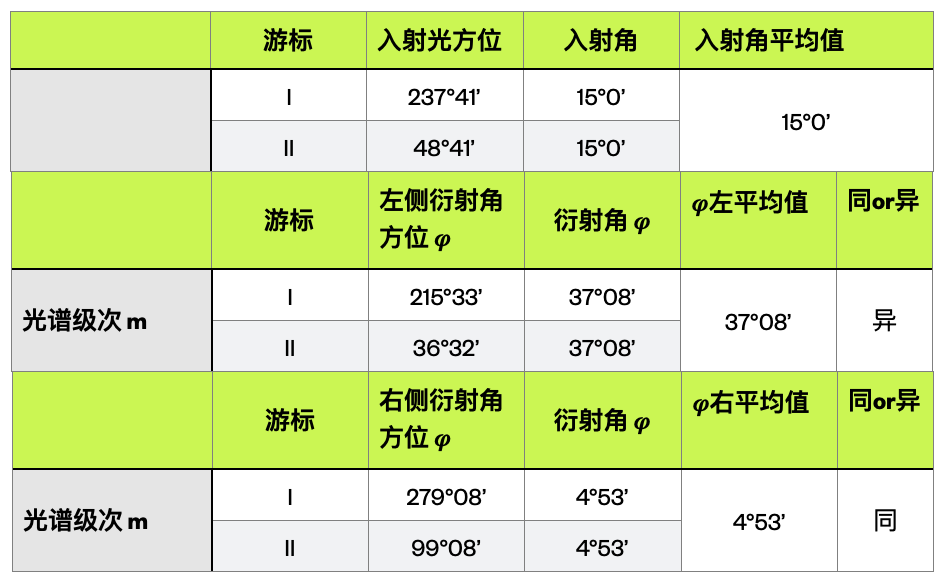
\includegraphics[width=0.8\linewidth]{./image/2.png}
% 	\caption{测量波长较短的黄线的波长} 
% 	\label{png:2}
% \end{figure}















\newpage
%%%%%%%%%%%%%%%%%%%%%%%%%%%%%%%%%%%%%%%%%%%%%%%%%%
%  参考文献
%%%%%%%%%%%%%%%%%%%%%%%%%%%%%%%%%%%%%%%%%%%%%%%%%%%%%%%%%%%%%%%%
%  参考文献按GB/T 7714-2015《文后参考文献著录规则》的要求著录. 
%  参考文献在正文中的引用方法:\cite{bib文件条目的第一行}

\renewcommand\refname{\heiti\wuhao\centerline{参考文献}\global\def\refname{参考文献}}
\vskip 12pt

\let\OLDthebibliography\thebibliography
\renewcommand\thebibliography[1]{
  \OLDthebibliography{#1}
  \setlength{\parskip}{0pt}
  \setlength{\itemsep}{0pt plus 0.3ex}
}

{
\renewcommand{\baselinestretch}{0.9}
\liuhao
\bibliographystyle{gbt7714-numerical}
\bibliography{./TempExample}
}


\end{document}
